\subsection{CU4 Registrar Entrada de Vehículo}
Pantalla que aparece al presionar el botón de 'Registrar Vehículo' en la visualización de agenda (figura \ref{fig:Pantalla Visualizar Menu - Vista de Escenarios}). Este formulario le solicita al usuario los siguientes campos: Número de Inventario, Descripción, Fecha de Entrada, Fecha de Salida y el Procedimiento que se le hará al vehículo. 
\\
Cuenta con dos botones en la parte inferior, uno para proceder a enviar el registro a la base de datos y otro para cancelar en caso de que el usuario así lo desee. 
\\
\begin{figure}[!h]
	\centering
	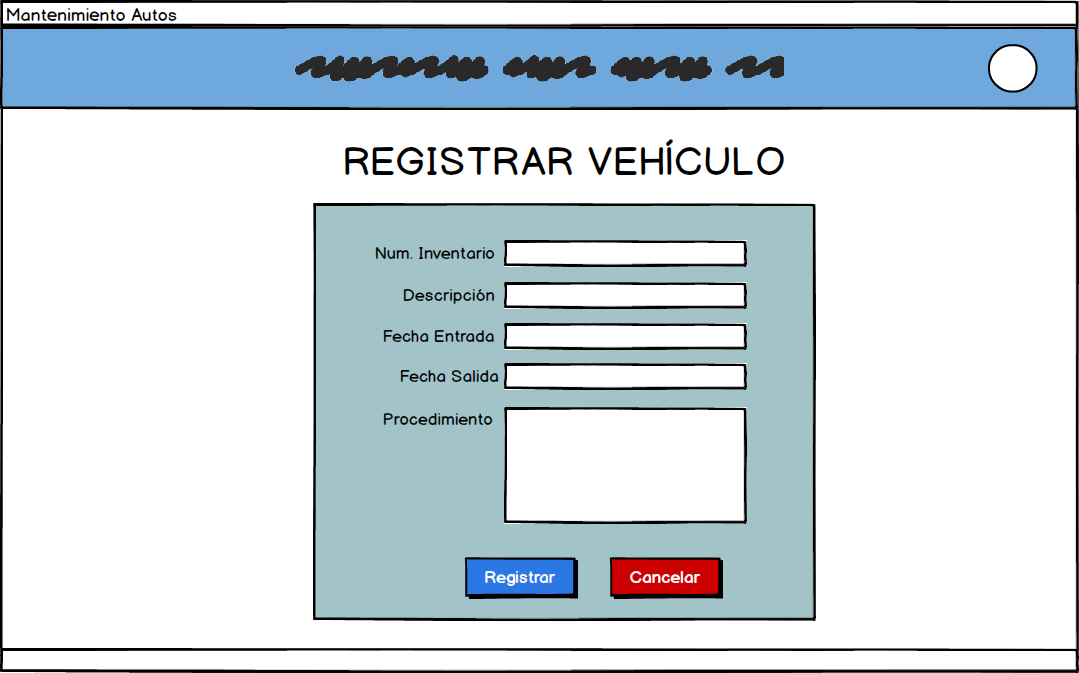
\includegraphics[width=0.9\textwidth]{./diseno/vescenarios/imagenes/registrarVehiculo}
	\caption{Pantalla Registrar Vehículo - Vista de Escenarios}
	\label{fig:Pantalla Registrar Vehículo - Vista de Escenarios}
\end{figure}
\\
En caso de que el usuario ingrese algún dato mal, es decir, que los campos no estén llenos o el formato de la información no es el correcto, aparecerá una alerta como la que se muestra a continuación (figura \ref{fig:Alerta2 - Vista de Escenarios}):
\begin{figure}[!h]
	\centering
	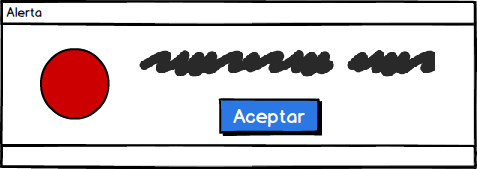
\includegraphics[width=0.4\textwidth]{./diseno/vescenarios/imagenes/alerta}
	\caption{Alerta Confirmación de Registro - Vista de Escenarios}
	\label{fig:Alerta2 - Vista de Escenarios}
\end{figure}
\clearpage